%%%%%%%%%%%%%%%%%%%%%%%%%%%%%%%%%%%%%%%%%%%%%%%%%%%%%%
\section{Neural network determination of the ZLP}
%%%%%%%%%%%%%%%%%%%%%%%%%%%%%%%%%%%%%%%%%%%%%%%%%%%%%
\label{sec:methodology}

In this section we present our strategy to parametrise, predict and subtract 
the zero-loss peak by means of machine learning.
%
As mentioned in the introduction, our strategy will be inspired by the 
NNPDF method~\cite{Rojo:2018qdd} originally developed in the context of high-energy physics
for studies of the quark and gluon substructure of the proton~\cite{Gao:2017yyd}.
%
The NNPDF approach has been successfully applied, among others, to
the determination of
unpolarised~\cite{DelDebbio:2007ee,Ball:2008by,Ball:2012cx,Ball:2014uwa,Ball:2017nwa}
and polarised parton distributions functions of protons, nuclear
parton distributions~\cite{AbdulKhalek:2019mzd,AbdulKhalek:2020yuc}, and the
fragmentation functions of partons into neutral and charged
hadrons~\cite{Bertone:2017tyb,Bertone:2018ecm}.
%
Neural networks benefit from the ability to parametrise 
multidimensional input data with nonlinear dependencies:
even with a single hidden layer, a neural network can reproduce arbitrary 
functional dependencies provided it has a large enough number of neurons.
%
We can therefore apply a similar procedure for the determination of the
functional dependence of the ZLP intensity. 

We note that recently several applications of machine learning
to transmission electron microscopy analyses 
in the context of material science have been
presented, see {\it e.g.}~\cite{Gordon:2020, Zhang:2019, Jany:2017, Ziatdinov:2017,10.1145/2834892.2834896,doi:10.1021/acsnano.7b07504,cite-key}.
%
Representative examples
include the automated identification
of structural information at the atomic scale~\cite{10.1145/2834892.2834896} 
and the extraction of chemical information
and defect classification~\cite{doi:10.1021/acsnano.7b07504}.
%
For the readout of EEL spectra specifically, 
machine learning has been put forward for the prediction
of spectral features in the core-loss regime~\cite{Kiyohara:2018}.
%
To the best of our knowledge, this is the first time that neural networks are used as 
unbiased background-removal interpolators and combined with 
Monte Carlo sampling to construct an estimate of the model uncertainties.\\

In this section, we discuss the parametrisation of the ZLP in terms of neural networks.
%
The ultimate goal is to create a model that is able to predict the contribution $I_{\rm ZLP}$
in the total intensity profile of any EEL spectrum recorded over a specimen, 
and subsequently to subtract this distribution from the spectrum to isolate the inelastic
scattering contributions.
%
In order to do so, we first need to develop a model that is able to predict the general
shape of the zero-loss peak as a function of its input parameters. 
%
For this we use in-vacuum zero-loss peak recordings, which function as a baseline to 
create this generic, multidimensional model.
%
In this regard we also
explain the Monte Carlo replica method, which is used to estimate and propagate the
uncertainties from the input data to the model predictions.
%
After this we move on to the training strategy on sample spectra: 
we explain how the method is modified to use it on spectra recorded over
WS$_2$ specimens and how one can select the hyper-parameters that appear in the model.


\subsection{ZLP parametrisation}
\label{sec:parametrisation}

Without any loss of generality, we can decompose the recorded intensity profile
in any EEL spectrum as
\be
\label{eq:IeelTot}
I_{\rm EEL}(\Delta E) =I_{\rm ZLP}(\Delta E) + I_{\rm inel}(\Delta E) \, ,
\ee
where $\Delta E$ is the measured electron energy loss; $I_{\rm ZLP}$ is the zero-loss
distribution arising both from instrumental origin and from elastic interactions; and
$I_{\rm inel}(\Delta E)$ contains the contributions from the electrons that have undergone
inelastic scattering with the specimen. 
%
It is the latter contribution that we're particularly interested in, but in order 
to get hold of it we need to disentangle it from the zero-loss contribution.
%
As shown by the representative example of Fig.~\ref{fig:EELS}, there are two limits
for which one can straightforwardly separate the two contributions.
%
The first is for sufficiently high energy losses, where
$I_{\rm ZLP}$ vanishes and $I_{\rm EEL} \to I_{\rm inel}$.
%
Secondly, in the region close to zero, all emission can be associated to
the ZLP such that $I_{\rm EEL}\to  I_{\rm ZLP}$.
%
It is the region in between that is of particular interest, 
the very-low-loss region where $I_{\rm ZLP}$ and $I_{\rm inel}$
become of comparable order of magnitude.

Our goal is to construct a parametrisation of $I_{\rm ZLP}$ based on artificial
neural networks, which we denote by $I_{\rm ZLP}^{\rm (mod)}$, which allows us to
extract the relevant inelastic contribution by subtracting the
contribution of the ZLP from the total EEL spectra:
\be
\label{eq:ZLPseparation}
I_{\rm inel}(\Delta E) \simeq I_{\rm EEL}(\Delta E) - I_{\rm ZLP}^{\rm (mod)}(\Delta E) \,.
\ee
Isolating $I_{\rm inel}$ from the total spectrum makes us able to exploit 
the physical information contained in the low-loss region.
%
Crucially, we aim to estimate and propagate all the relevant sources of uncertainty associated
both to the input data and to methodological choices. 
%
This helps us to verify our results and to separate lucky findings from real insights.\\

As discussed in Sect.~\ref{sec:eels}, the ZLP depends both
on the value of the electron energy loss $\Delta E$ as well as on the operating
conditions of the microscope, such as the electron beam energy $E_b$ and the exposure time
$t_{\rm exp}$.
%
Therefore we want to construct a multidimensional model which can theoretically take any number of relevant variables
as input, in order to reproduce the predicted zero-loss peak.
%
This means that in general Eq.~(\ref{eq:ZLPseparation}) can be written as
\be
I_{\rm inel}(\Delta E) = I_{\rm EEL}(\Delta E, E_{b},t_{\rm exp}, \ldots) - I_{\rm ZLP}^{\rm (mod)}(\Delta E, E_{b},t_{\rm exp}, \ldots) \, ,
\ee
where we note that the subtracted spectrum $I_{\rm inel}(\Delta E)$ should depend only on the energy loss, but not on the microscope parameters.
%
Ideally, the ZLP model should be able to accomodate as many input variables as possible.
%
The output of the ZLP model is parametrised by means of multi-layer feed-forward artificial neural networks.
This means that the predicted zero-loss peak intensity can be expressed as 
\be
\label{eq:ZLPmodelNN}
I_{\rm ZLP}^{\rm (mod)}(\Delta E, E_{b},t_{\rm exp}, \ldots)  = \xi^{(n_l)}_1(\Delta E, E_{b},t_{\rm exp}, \ldots) \, ,
\ee
where $\xi^{(n_l)}_1$ is the activation state of the single output neuron in the last
of the $n_l$ layers of the network. Here the $n_I$ inputs are the variables $\{ \Delta E, E_{b},t_{\rm exp}, \ldots \}$
that represent the relevant information about the operating conditions during the recording of the spectra.
%
Note that for this work, we have used spectra recorded under the known conditions $\{ \Delta E, E_{b},t_{\rm exp}\}$. 
%
This set of inputs could potentially be extended by including extra variables, 
{\it e.g.} arperture width, aberration correction and temperature. 
%
The neural network is then trained by means of supervised learning and nonlinear regression on these  
$n_I$ inputs, using the known corresponding ZLP intensities $I_{\rm ZLP}^{\rm (mod)}$ as training outcomes. 
%
Each iteration, the weights and thresholds of this neural network model are optimized
from the minimization of the error on this training dataset.\\

The number of hidden layers and neurons that is optimal is very task dependent and
should therefore be decided arbitrarily, 
there is no general rule of thumb. 
%
We have chosen to use an $n_I$-10-15-5-1 architecture with three hidden layers, wich corresponds to a total
number of 289~(271) free parameters for $n_I=3$~($n_I=1$) to be optimised.
%
However, we have verified that results are fairly independent of this exact choice;
we will elaborate on this later onwards.
  
%%%%%%%%%%%%%%%%%%%%%%%%%%%%%%%%%%%%%%%%%%%%%
\begin{figure}[H]
    \centering
    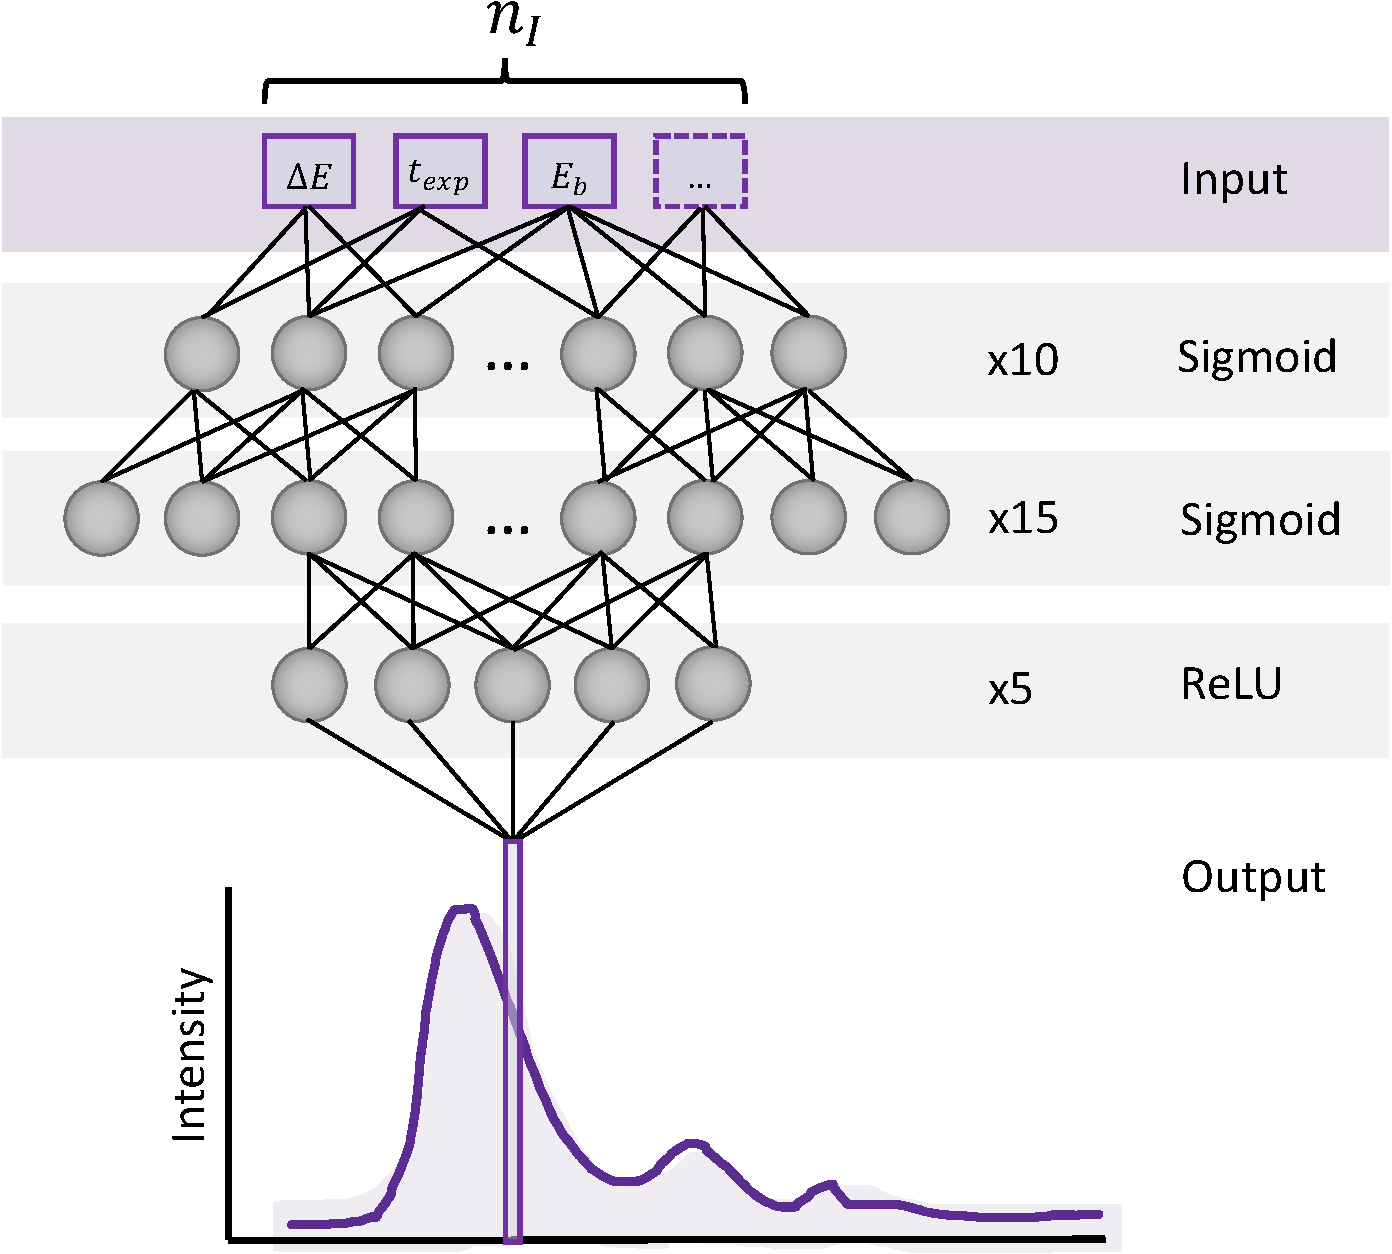
\includegraphics[width=99mm]{plots/architecture.pdf}
    \caption{Schematic representation of our ML model for the ZLP, Eq.~(\ref{eq:ZLPmodelNN}).
      %
      The input is an $n_I$-dimensional array containing $\Delta E$ and other
      operation variables of the microscope such as $E_b$ and $t_{\rm exp}$.
      %
      The output is the predicted value of the intensity of the zero-loss peak
      distribution associated to those specific input variables.
      %
      The architecture is chosen to be $n_I$-10-15-5-1, with sigmoid activation functions
      in all layers except for a ReLU in the output neuron.
    }
    \label{fig:architecture}
\end{figure}
%%%%%%%%%%%%%%%%%%%%%%%%%%%%%%%%%%%%%%%%%%%%%%%%%

A schematic representation of this model
is displayed in Fig.~\ref{fig:architecture}.
%
 The input is an $n_I$ array containing $\Delta E$ and the rest of
 operating variables of the microscope, and
 the output is the value of the intensity of the ZLP distribution
 associated to those inputs.
 %
 We use a sigmoid activation function for the three hidden layers and a ReLU
 for the final one.
 %
 The choice of ReLU for the final layer guarantees that our model for the ZLP
 is positive-definite, as required by general physical considerations: the intensity
 count can never be smaller than zero.
 %
 We have adopted a redundant architecture to ensure that the ZLP parametrisation
 is sufficiently flexible, which means that this way we guarantee that
 the network can over-fit on the training inputs.
 %
 However, the final results should be evaluated before the network starts overfitting,
 as described in Sect.~\ref{sec:nn}. 
 %
 This means that we need to define a suitable regularisation strategy, which 
 will be explained later onwards in Sect.~\ref{sec:training}.


\subsection{Uncertainty propagation}
\label{sec:uncertaintypropagation}

We discussed in Sect.~\ref{sec:eels} how
even for EEL spectra taken at identical operating conditions of the microscope,
in general the resulting ZLP intensity profiles will be different.
%
Also, the input data can be described by a large number of different neural 
network configurations, each with a different functional form of $I_{\rm ZLP}^{(\rm mod)}$
but representing the data equally well.
%
The Monte Carlo replica method can be used to estimate these two sources of 
uncertainties, introduced by the experimental data and the methodology,
and to propagate them to physical predictions.
%
The basic idea is twofold:
first, it is useful to represent problems with a possibility of non-gaussian errors
through the use of their central values and uncertainties, which are obtained from a Monte Carlo sample
as their averages and standard deviations.
%
Second, when a problem requires a reconstruction of discrete sampling without making assumptions on its 
functional form, neural networks are useful to work as unbiased interpolators. 
%
It is the combination of both techniques that explains the use of neural networks to separate a smooth
signal from background signals, while the MC samples handles the fluctuations within the data.

%%%%%%%%%%%%%%%%%%%%%%%%%%%%%%%%%%%%%%%%%%%%%%%
\begin{figure}[h]
    \centering
    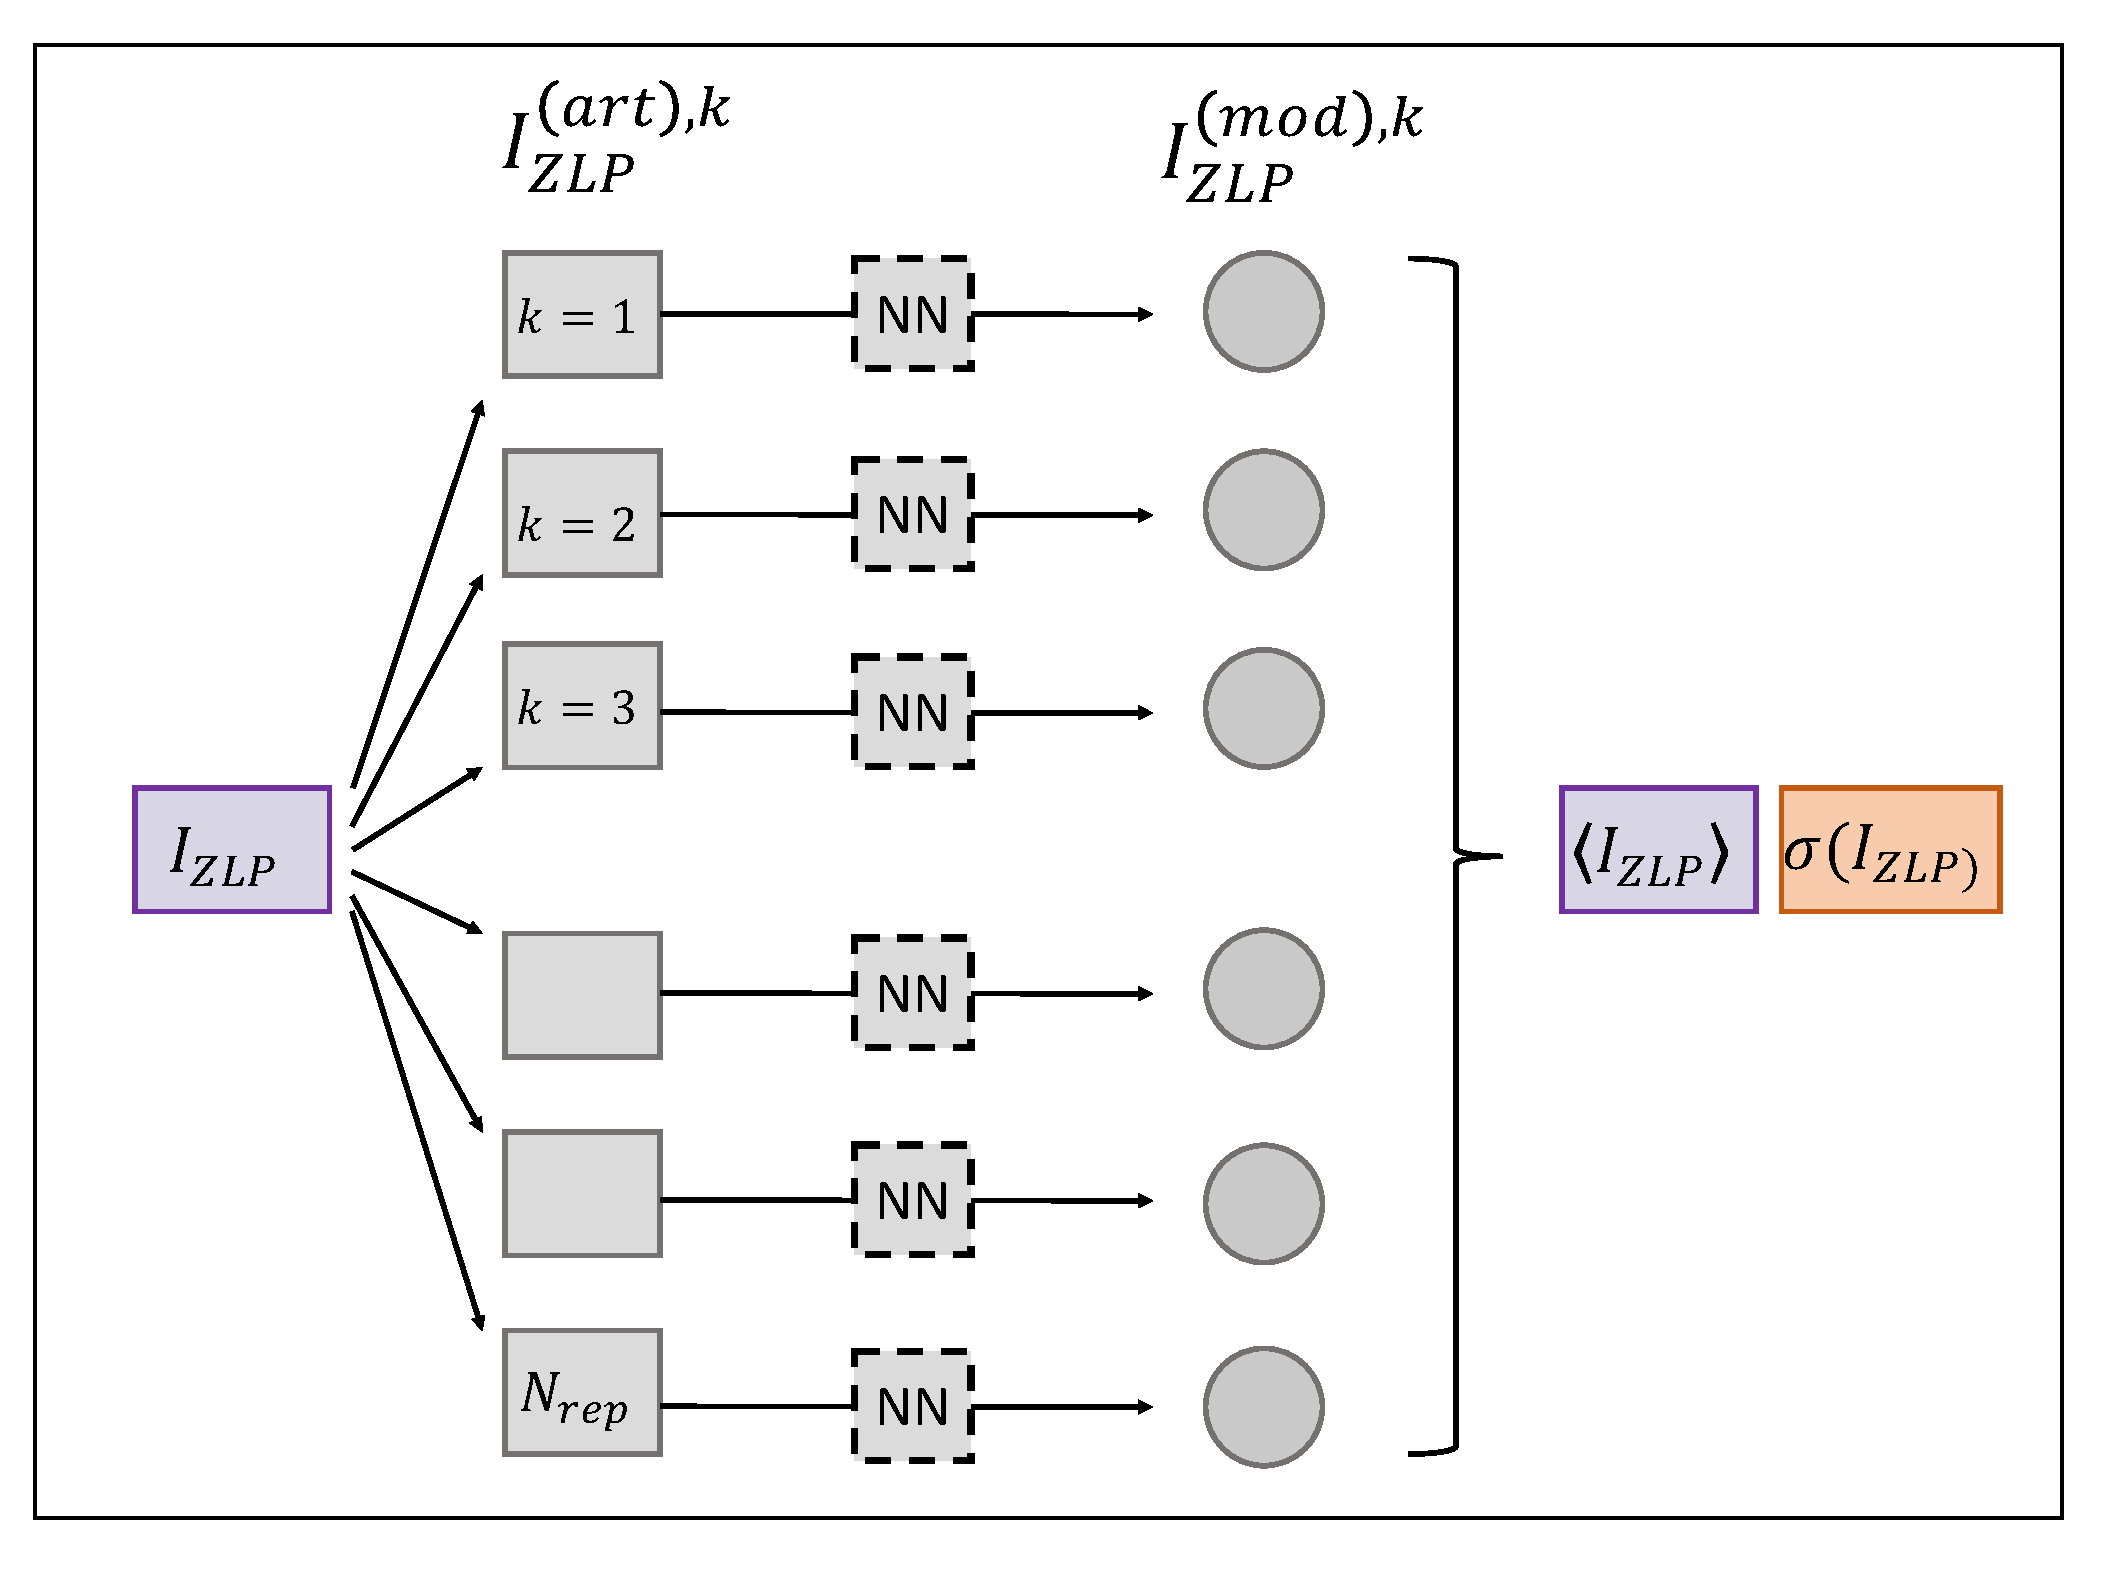
\includegraphics[width=0.7\textwidth]{plots/MCscheme.pdf}
    \caption{Representation of the Monte Carlo replica strategy. From the original set of training data,
    an ensemble of replicas is created from the experimental central values and uncertainties. 
    On each replica, an individual neural network is trained and a ZLP parametrisation is obtained.
    The total set of predictions is then used to calculate physical observables from the corresponding
    central values and uncertainties.}
    \label{fig:MCscheme}
\end{figure}
%%%%%%%%%%%%%%%%%%%%%%%%%%%%%%%%%%%%%%%%%%%%%%%%5

The MC strategy is schematically summarized in figure \ref{fig:MCscheme} and it involves two stages.
In the first, we generate an ensemble of replicas of the original training set using the
experimental central values and errors. 
%
Then, each replica is used to train 
an individual neural network, which thereby outputs a prediction of the ZLP.
%
Any physical observables can be calculated over the set of computed ZLP distributions.\\

Let us assume that we have $n_{\rm dat}$ independent measurements of the ZLP intensity, 
so our training dataset contains $n_{\rm dat}$ data points, all with different combinations of input parameters. 
%
The collective of inputs are given as $\{z_i\}$:
\be
I^{\rm (exp)}_{{\rm ZLP},i}\lp \{ z_i  \}\rp = I^{\rm (exp)}_{{\rm ZLP},i}\lp  \Delta E_i, E_{b,i}, t_{\rm exp,i},\ldots \rp
\,, \quad i=1,\ldots,n_{\rm dat} \, .
\ee

The Monte Carlo method is based on the generation
of a large number $N_{\rm rep}$ of Monte Carlo replicas of these original data points
by means of a multi-Gaussian distribution, where we use the central values and covariance matrices
from the input measurements. 
%
The strategy of the generation of Monte Carlo replicas goes as follows: we create for each original data point
($I^{\rm (exp)}_{{\rm ZLP},i}$) an ensemble of artificial pseudo points (replicas): 
\be
\label{eq:MCreplicaGen}
  I_{{\rm ZLP},i}^{{\rm (art)}(k)}  =  I^{\rm (exp)}_{{\rm ZLP},i} + r_i^{({\rm stat},k)}\sigma_i^{\rm (stat)}
  + \sum_{j=1}^{n_{\rm sys}} r_{i,j}^{({\rm sys},k)} \sigma_{i,j}^{\rm (\rm sys)} \,, \quad \forall i
  \,, \quad k=1,\ldots,N_{\rm rep} \,.\,\, \,
  \ee
  where $\sigma_i^{\rm (stat)}$ and $\sigma_{i,j}^{\rm (\rm sys)}$ represent the statistical
  and systematic uncertainties (the latter divided into  $n_{\rm sys}$ fully point-to-point correlated
  sources) and $\{r_i^{(k)}\}$ are Gaussianly distributed random numbers.
  %
In the end, each $k$-th replica contains exactly
as many data points as the original set.

In our case we have no information on experimental correlations between the measurements and
for this reason we assume that there is only one single source of point-by-point systematic
uncertainty, which is uncorrelated. 
%
  Should in the future correlations became available, it would be straightforward to extend
  our model to that case.
%
In other words, to each data point we associate an individual uncertainty and we 
discard covariances between datapoints, which means that we drop the last term in Eq.~(\ref{eq:MCreplicaGen})
and it reduces to
\be
\label{eq:MCreplicaGen2}
  I_{{\rm ZLP},i}^{{\rm (art)}(k)}  =  I^{\rm (exp)}_{{\rm ZLP},i} + r_i^{({\rm stat},k)}\sigma_i^{\rm (stat)}.
\ee

These statistical errors on the training data can be derived by means of what is called
equal width discretization (EWD) and it works as follows.
%
The input measurements will be composed in general on subsets of EEL
spectra taken with identical operating conditions.
%
For example, we have one specific set of $N_{sp}$ spectra all recorded with 
the same exposure time and beam energy. 
%
Since the range of $\Delta E$ over which the spectra have been recorded
is usually not the same in each case, first of 
we uniformise a common binning in $\Delta E$ with $n_{\rm dat}$ entries.
%
Then we evaluate the total experimental uncertainty in one of these bins as
\begin{equation}
\label{eq:sigmaiexp}
\sigma_i^{\rm (exp)} = \lp \frac{1}{N_{\rm sp}-1} \sum_{l=1}^{N_{\rm sp}}
\lp I_{{\rm ZLP},i}^{ ({\rm exp}),l}  - \la I_{{\rm ZLP},i}^{ ({\rm exp})}\ra_{N_{\rm sp}} \rp \rp^{1/2} \, ,\,
i=1,\ldots, n_{\rm dat} \, ,
\end{equation}
that is, $\sigma_i^{\rm (exp)}$ is the standard deviation in bin $i$ calculated over the $N_{\rm sp}$ spectra.
%
This uncertainty is separately evaluated for each set of microscope operation conditions
for which data available.
%
The value of the number of generated MC replicas, $N_{\rm rep}$, should be chosen such that the set of replicas 
models accurately the probability distribution of original training data.
%
%%%%%%%%%%%%%%%%%%%%%%%%%%%%%%%%%%%%%%%%%%%%%%%
\begin{figure}[t]
    \centering
    \includegraphics[width=0.99\textwidth]{plots/MC-Copy1.pdf}
    \caption{Comparison between the original experimental central values
      $I_{\rm ZLP,i}^{\rm exp}$ (left panel) and the corresponding statistical
      uncertainties $\sigma_i^{(\rm stat)}$ with the results of averaging over
      a sample of $N_{\rm rep}$ Monte Carlo replicas generated by means of
      Eq.~(\ref{eq:MCreplicaGen}), for different values of
      $N_{\rm rep}$.
      }
    \label{fig:MC}
\end{figure}
%%%%%%%%%%%%%%%%%%%%%%%%%%%%%%%%%%%%%%%%%%%%%%%%5

To verify that this is the case,
Fig.~\ref{fig:MC} displays a comparison between the original experimental central values
$I_{{\rm ZLP},i}^{\rm (exp)}$ (left) and the corresponding 
total uncertainties $\sigma_i^{(\rm exp)}$ (right panel) with the results of averaging over
a sample of $N_{\rm rep}$ Monte Carlo replicas generated by means of
Eq.~(\ref{eq:MCreplicaGen}) for different numbers of replicas.
%
We find that $N_{\rm rep}=500$ is a value that ensures that both
the central values and uncertainties are reasonably well reproduced,
and we adopt it in what follows.


\subsection{Training strategy}
\label{sec:training}

The training of the neural-network model for the ZLP peak differs between
the cases of EEL spectra taken on vacuum,
where by construction $I_{\rm EEL}(\Delta E) =I_{\rm ZLP}^{\rm (mod)}(\Delta E)$,
and for spectra taken on samples. 
%
In fact, EEL spectra taken in the vacuum but close
to the sample might still receive inelastic contributions coming from the specimen.
%
When we talk about vacuum spectra, we consider exclusively those taken 
reasonably far from the surface of the analysed nanostructures.
%
In the case of spectra recorded on specimens, we need to find a training strategy to make predictions
about the ZLP distribution in the low-loss regime, while we can not directly
train on data in this region.
%
As indicated by Eq.~(\ref{eq:ZLPseparation}), in order to avoid
biasing the results it is important to ensure that the model is trained only on the region of the spectra
where the ZLP dominates over the inelastic scatterings.
%
Then we can make predictions in the extrapolation regime based on these 
training parameters.
%
We now describe the training strategy that is adopted in both cases.

\paragraph{Training of vacuum spectra.}
%
For each of the $N_{\rm rep}$ generated Monte Carlo replicas, we train an independent
neural network as described in Sect.~\ref{sec:parametrisation}.
%
Fitting the neural networks parameters to the data is performed by minimisation of a
figure of merit (error function), defined as:
\begin{equation}
  \label{eq:chi2}
\begin{centering}
  E^{(k)}\lp \{\theta^{(k)}\}\rp = \frac{1}{n_{\rm dat}}\sum_{i=1}^{n_{dat}}\left(\frac{ I_{{\rm ZLP},i}^{{\rm (art)}(k)} -
  I_{{\rm ZLP},i}^{{\rm (mod)}}\lp \{\theta^{(k)}\}\rp }{\sigma_i^{(\rm exp)}}\right)^2, 
\end{centering}
\end{equation}

which is the $\chi^2$ per data point comparing each replicated ZLP intensity
with the corresponding model prediction.
%
In this expression $E^{(k)}\lp \{\theta^{(k)}\}\rp$ is the error for the values 
$\{\theta^{(k)}\}$ of the network weights and thresholds;
$I_{{\rm ZLP},i}^{{\rm (art)}(k)}$ is the $k$-th replica for the ZLP 
intensity and $I_{{\rm ZLP},i}^{{\rm (mod)}}$ is the model prediction on this
replica; and ${\sigma_i^{(\rm exp)}}$ again represents the error
associated to this experimental data point.\\

The chi-squared method is the cornerstone of almost all fitting, 
as it is an intuitively reasonable measure of how well the predictions fit the data. 
%
If the model predictions are all within one standard deviation from the data, 
then the $\chi^2$ per data point takes a value roughly equal to 1. 
%
In general, if $\chi^2/n_{dat}$ is of the order 1, we can say that the 
fit is a good approximation to the real data. 

In order to speed up the neural network training process, prior to the optimisation
all inputs and outputs are scaled to lie between $[0.1, 0.9]$ before
being feed to the network.
%
This preprocessing facilitates that
the neuron activation states will typically
lie close to the linear region of the sigmoid activation function.\\

The contribution to the figure of merit from the input experimental data, Eq.~(\ref{eq:chi2}),
needs in general to be complemented with that of theoretical constraints on the model.
%
For instance, when determining nuclear parton distributions~\cite{AbdulKhalek:2020yuc}, one needs to
extend Eq.~(\ref{eq:chi2}) with Lagrange multipliers to ensure that both the $A=1$ proton boundary
condition and the cross-section positivity are satisfied.
%
In the case at hand, our model for the ZLP should satisfy the constraint that $I_{\rm ZLP}(\Delta E)\to 0$
when $|\Delta E| \to \infty$, since far from $\Delta E\simeq 0$ the contribution from the ZLP
is completely negligible.
%
In order to implement this constraint, we add $n_{pd}$ pseudo-data points to the training dataset 
"far" away from the ZLP and we modify
the figure of merit Eq.~(\ref{eq:chi2}) accordingly,
\be
\label{eq:chi2modified}
E^{(k)}\lp \{\theta^{(k)}\}\rp \to E^{(k)}\lp \{\theta^{(k)}\}\rp +
\lambda \sum_{i'=1}^{n_{pd}}\left(
  I_{{\rm ZLP},i'}^{{\rm (mod)}}\lp \{\theta^{(k)}\}\rp \right)^2, 
  \ee
  where $\lambda$ is a Lagrange multiplier whose value is tuned to ensure that the $I_{\rm ZLP}(\Delta E)\to 0$
  condition
  is satisfied without affecting the description of the training dataset.
  %
  In other words, we add a contribution to the error function coming from these pseudo points in the
  higher-loss regime, making sure that the optimization of the error function also takes into account
  the fact that at higher losses the intensity should vanish.
  %
  However, when calculating the overall fit quality after training, we do not include the second term
  on the right-hand side of Eq.~(\ref{eq:chi2modified}) in the evaluation of the figure of merit, 
  as these "fake" datapoints do not give any physical
  information about the original dataset whatsoever.

  The pseudo-data points are added in the region $\lc \Delta E_{\rm pd}^{\rm (min)},
  \Delta E_{\rm pd}^{\rm (max)}\rc$, and symmetrically for negative energy losses.
  %
The value of $\Delta E_{\rm pd}^{\rm (min)}$
can be determined automatically by evaluating the ratio $\mathcal{R}_{\rm sig}$ between the central
experimental intensity and the total uncertainty in each data point,
\be
\label{eq:pdlocation}
\mathcal{R}_{\rm sig}(\Delta E_i)\equiv \frac{I_{{\rm ZLP}}^{(\rm exp)}(\Delta E_i)}{\sigma^{(\rm exp)}(\Delta E_i)} \, ,
\ee
which corresponds to the statistical significance for the $i$-th bin of $\Delta E$ to differ from the null hypothesis
(zero intensity) taking into account the experimental uncertainties.
%
For sufficiently large energy loss this ratio approaches 1, which indicates that we are essentially
fitting statistical noise. 
%
In order to avoid this and only fit data that is different from zero within errors, we determine the value
of $\Delta E_{\rm pd}^{\rm (min)}$ from the condition that $ \mathcal{R}_{\rm sig}(\Delta E_i) \simeq$ 1. 
%
We keep the training data in the region $\Delta E \le \Delta E_{\rm pd}^{\rm (min)}$ and the pseudo-data
points are added for $\lc \Delta E_{\rm pd}^{\rm (min)}, \Delta E_{\rm pd}^{\rm (max)}\rc$. 
%
The value of $\Delta E_{\rm pd}^{\rm (max)}$ can be chosen arbitrarily and can be as large as necessary
to ensure that $I_{\rm ZLP}(\Delta E)\to 0$ as $|\Delta E| \to \infty$.

We note that another important physical condition on the ZLP model, namely its positivity
(since in EEL spectra the intensity is just a measure of the number of counts in the
detector for a given value of the energy loss) is automatically satisfied since
we use a ReLU activation function for the last layer.
%
A further obvious requirement is that the best fit is independent of any assumptions 
made about the ZLP distribution. 
%
This requirement can be met by making sure the parametrisation is redundant: 
the size of the neural network used, and therefore the number of optimizable parameters, 
is much larger than the minimum required in order to reproduce the data. 
%
This redundancy can be verified {\it a posteriori}, that results are independent of 
the size and architecture of the neural network.\\

In this work we adopt the {\tt TensorFlow} neural-net libraries to assemble
the architecture illustrated in Fig.~\ref{fig:architecture}.
%
Before training, all weights and biases are initialized in a non-deterministic order
by the built-in global variable initializer. 
%
The optimisation of the figure of merit Eq.~(\ref{eq:chi2modified}) is carried
out by means of stochastic gradient descent (SGD) combined with backpropagation. The
specific SGD optimizer used is the Adam algorithm.
%
The hyper-parameters of the optimisation algorithm such as the learning rate
have been adjusted to ensure proper learning is reached in the shortest amount
of time possible.
%
Given that we have a extremely flexible parametrisation, one should be careful
to avoid overlearning the input data.
%
Here over-fitting is avoided by means of a cross-validation stopping criterion.
%
We separate the input data into training a validation subsets, with a 80\%/20\% splitting
which partition varies randomly for each Monte Carlo replica.
%
We then run the optimiser for a very large number of iterations and store both
the state of the network and the value
of the figure of merit Eq.~(\ref{eq:chi2}) restricted to the validation
dataset, $E^{(k)}_{\rm val}$ (which is not used for the training).
%
We are not looking for the absolute minimum of the error function, 
but we rather search for an optimal stopping point to avoid overfitting. 
%
At this optimal stopping point, it reproduces the information contained in the dataset, 
but not its statistical fluctuations.
%
This point can be determined by the formulation of a stopping criterion, 
making it possible to, once the network completed the training, 
choose the parametrization of the network weights right before it 
entered the overlearning regime. 
%
The optimal stopping point is determined  for each replica
by keeping track of the figure of merit, which typically evolutes
as depicted in Fig.~\ref{fig:costs}. 
%
The specific network configuration that leads to the deepest minimum of $E^{(k)}_{\rm val}$
is chosen after training, that's why it is called look-back stopping, 
a method that has been widely used in the context
of neural networks.
%
The number of epochs should be chosen high enough to reach for each replica 
the absolute minimum of $E^{(k)}_{\rm val}$, 
rather than a local minimum.
For this work we need approximately 40,000 epochs to guarantee overlearning.
%
This corresponds to a serial running time of 60 seconds per replica when running the optimization on a 
single CPU for a set of 500 datapoints.
%
Once the training of all the $N_{\rm rep}$ neural network models for the ZLP has been carried
out as specified above, we quantify the overal fit quality of the model by computing the
$\chi^2$ defined as
\begin{equation}
  \label{eq:chi2_final}
\begin{centering}
  \chi^2 = \frac{1}{n_{\rm dat}}\sum_{i=1}^{n_{dat}}\left(\frac{ I_{{\rm ZLP},i}^{{\rm (exp)}} -
 \la I_{{\rm ZLP},i}^{{\rm (mod)}}\ra_{\rm rep} }{\sigma_i^{(\rm exp)}}\right)^2, 
\end{centering}
\end{equation}
which is the analog of Eq.~(\ref{eq:chi2_final}) now comparing the average model prediction
to the original experimental data values.
%
A value $\chi^2 \simeq 1$ indicates that a satisfactory description of the experimental data,
within the corresponding uncertainties, has been achieved.
%
Note that in realistic scenarios $\chi^2$ can deviate from unity, for instance when
some source of correlation between the experimental uncertainties has been neglected
or when the errors on the data points have been over- or underestimated.


\paragraph{Training of sample spectra.}

The training strategy in the case of EEL spectra taken on samples (rather than on vacuum) must be adjusted
to account for the fact that the input data set, Eq.~(\ref{eq:IeelTot}), receives contributions
both from the ZLP and from inelastic scatterings.
%
To avoid biasing the ZLP model, we should make sure to include only the former contributions 
in the training dataset.
%
Else, if we were to train the neural network on data that contains also inelastic contributions,
subsequent subtraction to the EEL spectra would make us lose important information.

We can illustrate the situation at hand with the help of a toy model for the low-loss
region of EEL spectra, represented in
Fig.~\ref{fig:EELS_toy}.
%
Let us use a general assumption that the ZLP is described by a 
Gaussian distribution with a standard deviation of $\sigma_{\rm ZLP}=0.3$ eV,
and that the contribution from the
inelastic interactions with the sample can be approximated in the low-loss
regime by $I_{\rm inel}(\Delta E)\propto \lp \Delta E - E_{\rm bg}\rp^b$ with $E_{\rm bg}=1.5$
and $b=0.5$. 
%
The motivation for this
choice will be explained in Sect.~\ref{sec:results_sample}.
%
We display the separate contributions from $I_{\rm ZLP}$
and $I_{\rm inel}$, as well as the total intensity,  
with the inset showing the values of the corresponding derivatives, $dI/d\Delta E$.

%%%%%%%%%%%%%%%%%%%%%%%%%%%%%%%%%%%%%%%%%%%%%
\begin{figure}[t]
    \centering
    \includegraphics[width=0.7\textwidth]{plots/Toy.pdf}
    \caption{A toy model for a generic EEL spectrum and its
      derivatives (in the inset).
      %
      We show the separate contributions from $I_{\rm ZLP}$
      and $I_{\rm inel}$ as well as their sum.
      %
      We indicate the two regions used for the model training ($I$ and $III$),
      while the trained model is interpolated to region $II$, 
      defined for $\Delta E_I \le \Delta E \le \Delta E_{II}$.}
    \label{fig:EELS_toy}
\end{figure}
%%%%%%%%%%%%%%%%%%%%%%%%%%%%%%%%%%%%%%%%%%%%%%%%%

The toy model of Fig.~\ref{fig:EELS_toy} is sufficiently general to draw
a number of useful considerations concerning the relation between $I_{\rm ZLP}$ and $I_{\rm inel}$
in realistic spectra:

\begin{itemize}

\item The ZLP intensity, $I_{\rm ZLP}(\Delta E)$, is a monotonically decreasing function
  and thus its derivative is always negative.

\item  The first local minimum of the total spectrum, $dI_{\rm EELS}/d\Delta E|_{\Delta E_{\rm min}}=0$, corresponds
  to a value of $\Delta E$ for which the contribution from the inelastic emissions is already
  significant.

\item The value of $\Delta E$ for which $I_{\rm inel}$ starts to contribute to the total spectrum
  corresponds to the position where the intensity derivatives in-sample and in-vacuum  start to differ.
  %
  We note that a direct comparison between the overal magnitude of the sample and vacuum ZLP
  spectra is in general not possible, as explained in Sect.~\ref{sec:eels}. 
\end{itemize}

These considerations suggest that when training the ML model on EEL spectra taken on samples,
the following categorisation of training regions should be adopted:

\begin{enumerate}

\item For small energy losses such that $\Delta E \le \Delta E_I$ (region $I$),
  the model training  proceeds in the same way as for the vacuum case
  via the minimisation of Eq.~(\ref{eq:chi2}).

\item  
  For $\Delta E \ge \Delta E_{II}$ (region $III$), we use instead Eq.~(\ref{eq:chi2modified})
  without the contribution from the input data, since for such values
  of $\Delta E$ one has that $I_{\rm inel}\gg I_{\rm ZLP}$.
  %
  In other words, we only train on the pseudo data and therefore
  the only information that region $III$ provides
  on the model is the one arising from the implementation
  of the constraint that $I_{\rm ZLP}(\Delta E\to \infty)\to 0$.

\item The EELS data in region $II$, defined by $\Delta E_I \le \Delta E \le \Delta E_{II}$,
  is excluded from the training dataset, given that in this region the contribution to $I_{\rm EEL}$
  coming from $I_{\rm inel}$ is already significant.
  %
  The model predictions in this regime are obtained from an interpolation
  of the predictions obtained in regions $I$ and $III$.

\end{enumerate}

This classification introduces two new hyper-parameters of our model, $\Delta E_I$ and
$\Delta E_{II}$, that need to be specified before the training.
%
They should satisfy $\Delta E_I \le \Delta E_{\rm min}$ and $\Delta E_{II} \ge \Delta E_{\rm min}$,
with $\Delta E_{\rm min}$ being the position of the first local minimum of $I_{\rm EEL}$.
%
Let's interpret this physically: $\Delta E_{\rm min}$ is the first local minimum, which means that 
the inelastic contributions are significantly present.
%
Training on data with energy loss higher than this value, we are sure that our training data includes
at least some amount of inelastic scatterings.
%
Therefore, it is certain that we need to cut the training data already at a lower energy loss,
so $\Delta E_I \le \Delta E_{\rm min}$.
%
As indicated by the toy spectra of Fig.~\ref{fig:EELS_toy}, a suitable value for $\Delta E_{I}$
would be somewhat above the onset of the inelastic contributions: this way we maximise
the amount of training data while ensuring that $I_{\rm EEL}$ is still dominated
by $I_{\rm ZLP}$.\\

We can use the derivatives of the spectra, $dI_{\rm EEL}/d\Delta E$, to select suitable minimum and
maximum values for $\Delta E_I$. 
%
Using first and second derivatives is an often-used feature extraction method to achieve a relatively 
high accuracy with a low computational complexity. 
%
In an ideal microscope the electron beam would be perfectly monochromatic, 
correspondingly the ZLP would appear as a delta function in an EEL spectrum \cite{Rafferty:2000}. 
%
In practice the ZLP has a finite width defining the energy resolution of the system. 
%
Concerning $\Delta E_I $, its minimum possible value is selected as the value where the derivate taken on the sample
data start to different significantly as compared to those spectra taken on vacuum.
%
This value is obtained by looking at the ratio of the derivatives of the spectra compared to the vacuum derivatives:
\be
R_{dI/d \Delta E} =  \left( \frac{dI_{\rm ZLP}/d\Delta E}{dI_{\rm EEL}/d\Delta E}\right). 
\ee
%
For low energy losses this ratio equals 1, which means that in the low-loss regime
the spectra recorded in vacuum and on specimens behave similar.
%
However, at some energy loss $\Delta E_{I,min}$ the
sample spectrum stops monotonically decreasing and the ratio deviates from 1. 
%
It is this point where the contributions from the sample start to change the shape of
the ZLP distribution and we can use this measure to mark the transition from 
regime I to regime II in Fig.~\ref{fig:EELS_toy}.
%
We know that the hyper-parameter $\Delta E_I$ should satisfy 
$\Delta E_{I,min} \le \Delta E_I \le \Delta E_{\rm min}$,
which corresponds to the region where $R_{dI/d \Delta E} \ne  1$ and $R_{dI/d \Delta E} \ge 0$.
%
The neural network will be trained on a range of different $\Delta E_I$ values within this interval,
and the optimal choice will be determined {\it a posteriori} from the results.
%
Also, generating results for different values of $\Delta E_I$ makes us able to 
cross-validate on the stability of our results regardless of the exact choice of this
hyperparameter.

Another important difference as compared to the training of the vacuum spectra is that each of the sample
spectra will have different values of $\Delta E_{\rm min}$ and thus of $\Delta E_I$. 
%
For this reason we calculate $\Delta E_{\rm min}$  for each of the sample spectra and we use the highest of these
as the maximum value for the hyper-parameter $\Delta E_I$. 
%
As we determine the best choice of $\Delta E_I$ after training for each of the spectra separately, 
we are sure to capture all suitable results and select the best value for each individual spectrum. \\

Concerning $\Delta E_{II}$, its minimum value should mark the region where $I_{\rm ZLP}(\Delta E\to \infty)\to 0$. 
%
It is the value where we start adding pseudo-data, so $\Delta E_{II}$ = $\Delta E_{\rm pd,min}$.
%
In order to implement this constraint, similar to the previous section (Eq.~(\ref{eq:pdlocation}))
we look at the ratio 
$\mathcal{R}_{\rm sig}(\Delta E_i)$ to determine the energy loss $\Delta E_{\rm pd}$ at 
which the contributions from the vacuum-recorded ZLP vanish. 
%
As a measure, we use the energy loss value where the ratio $\mathcal{R}_{\rm sig}(\Delta E_i)$ drops below 1,
as in this regime we would be fitting statistical noise.
%
We set the value of $\Delta E_{II}$ equal to this energy loss and add pseudo-data points for $\Delta E \ge \Delta E_{II}$.
%
Note that in this region the intensity of the ZLP is several orders of magnitude smaller than the intensity 
of the elastic emissions and therefore the exact choice of $\Delta E_{II}$ does not listen too closely.\\

Now that we have determined our strategy for the parametrisation of the ZLP, we move on to present the results,
first on vacuum recorded data and afterwards on specimen data.
